\documentclass[12pt, a4paper]{article}
\usepackage[spanish]{babel}
\usepackage[utf8]{inputenc}
\usepackage{graphicx}

\begin{document}

\begin{titlepage}
    \centering
    {\huge \textbf{Configuración del entorno de desarrollo de Python y texto sobre la relevancia técnica de Python en la IA}} \\[1cm]
    {\Large Actividad} \\[2cm]
    
    {\large Alumno: Angel Gabriel Coronado Sánchez} \\[1cm]
    {\large Asignatura: Fundamentos de la Inteligencia Artificial} \\[1cm]
    {\large Fecha: \today}
    
    \vfill
    {\large Universidad Politécnica de Victoria}
\end{titlepage}

\section{Evidencia de uso del entorno elegido}

\begin{figure}[h]
    \centering
    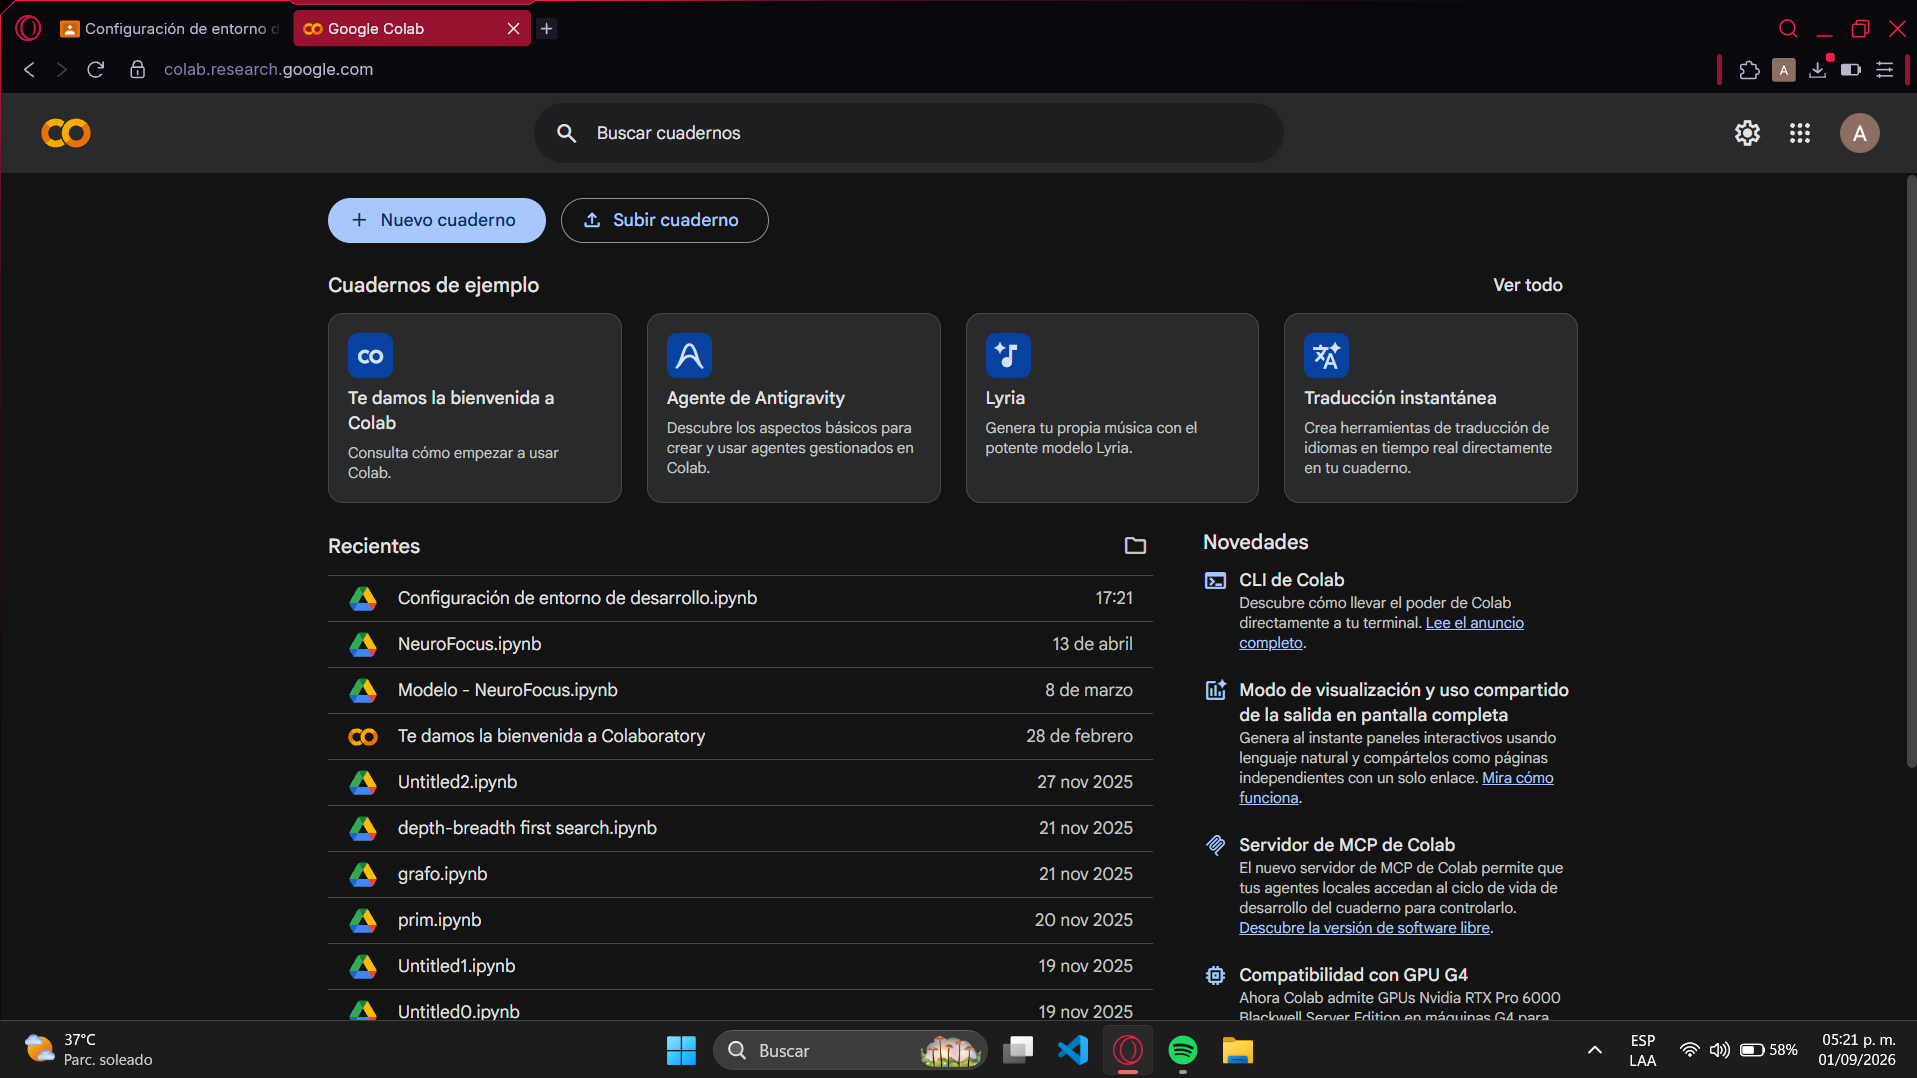
\includegraphics[width=0.79\textwidth]{img/entorno.png}
    \caption{Captura de pantalla del entorno elegido (Google Colab).}
    \label{fig:entorno}
\end{figure}

\section{Evidencia de ejecución de prueba de importación de librerías}

\begin{figure}[h]
    \centering
    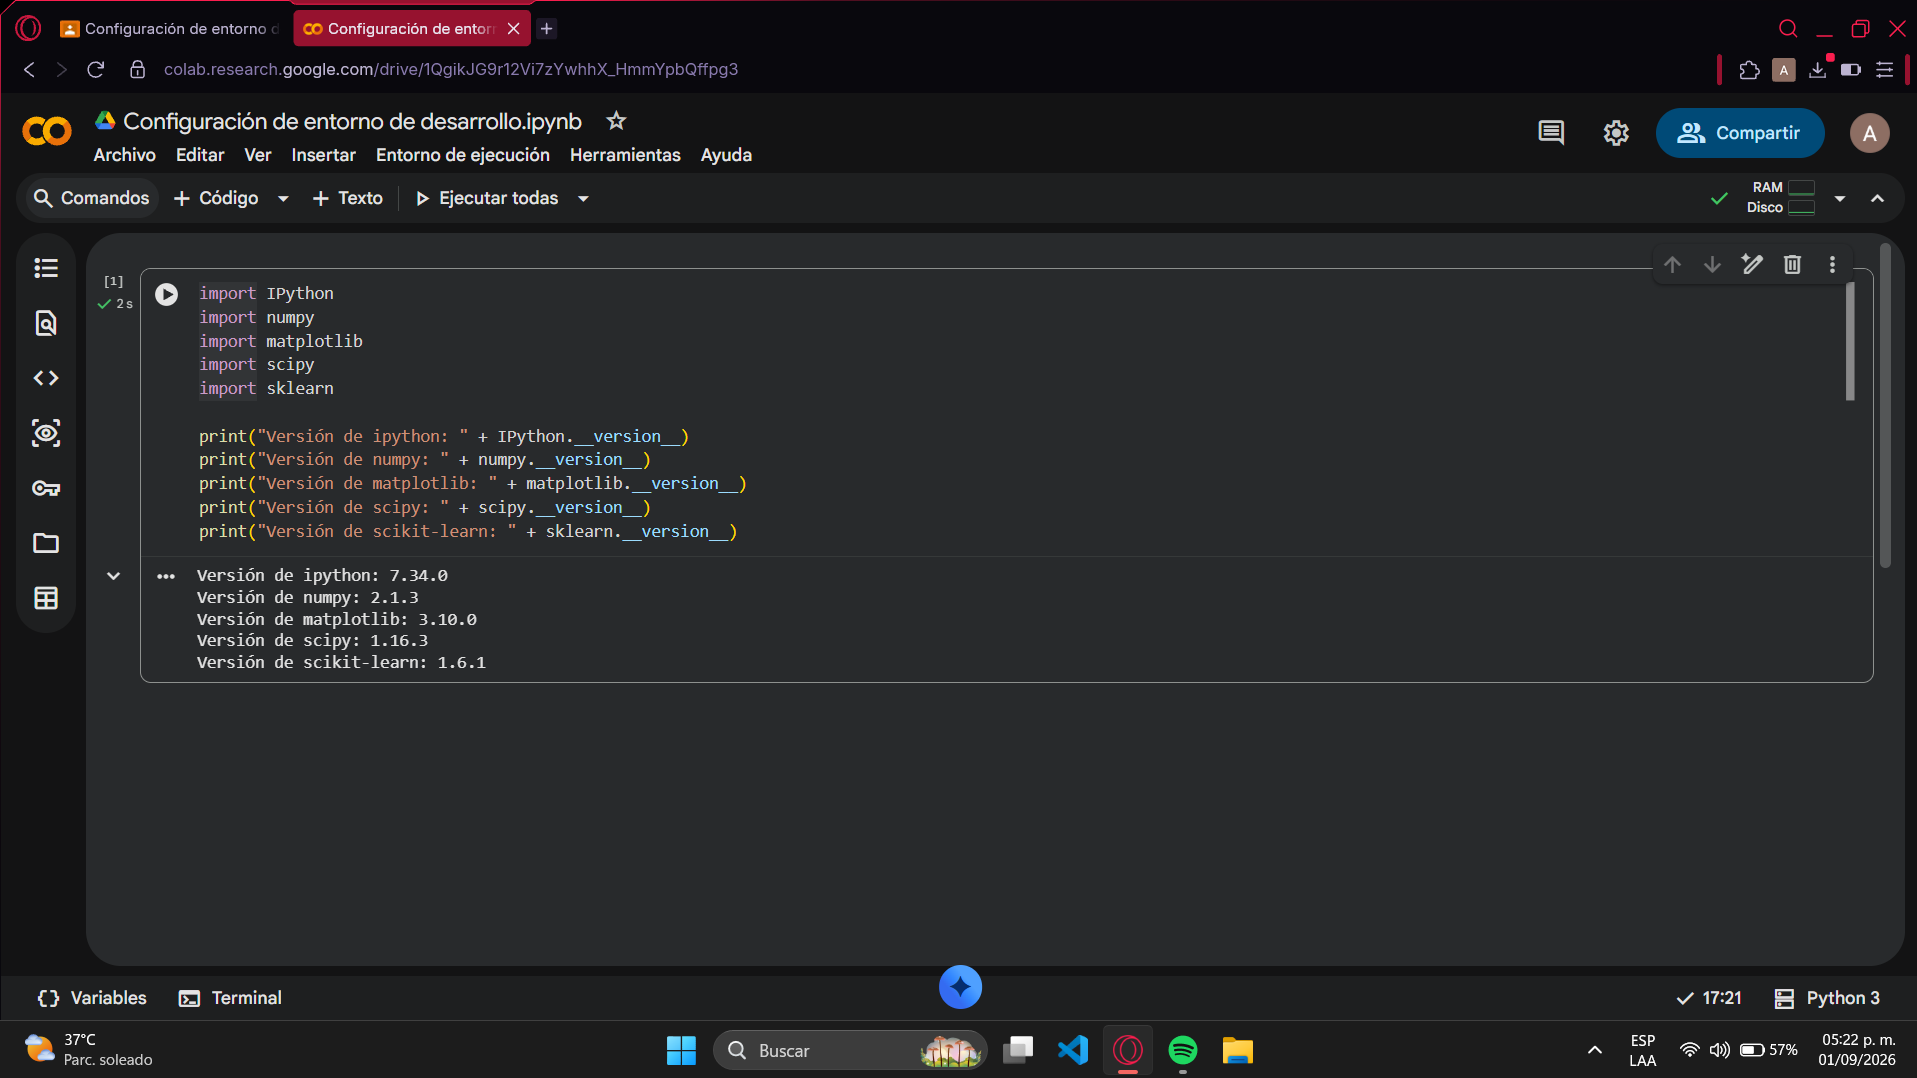
\includegraphics[width=0.79\textwidth]{img/prueba.png}
    \caption{Captura de pantalla de la prueba de importación de librerías.}
    \label{fig:prueba}
\end{figure}

\section{Texto de investigación}

\begin{figure}[h]
    \centering
    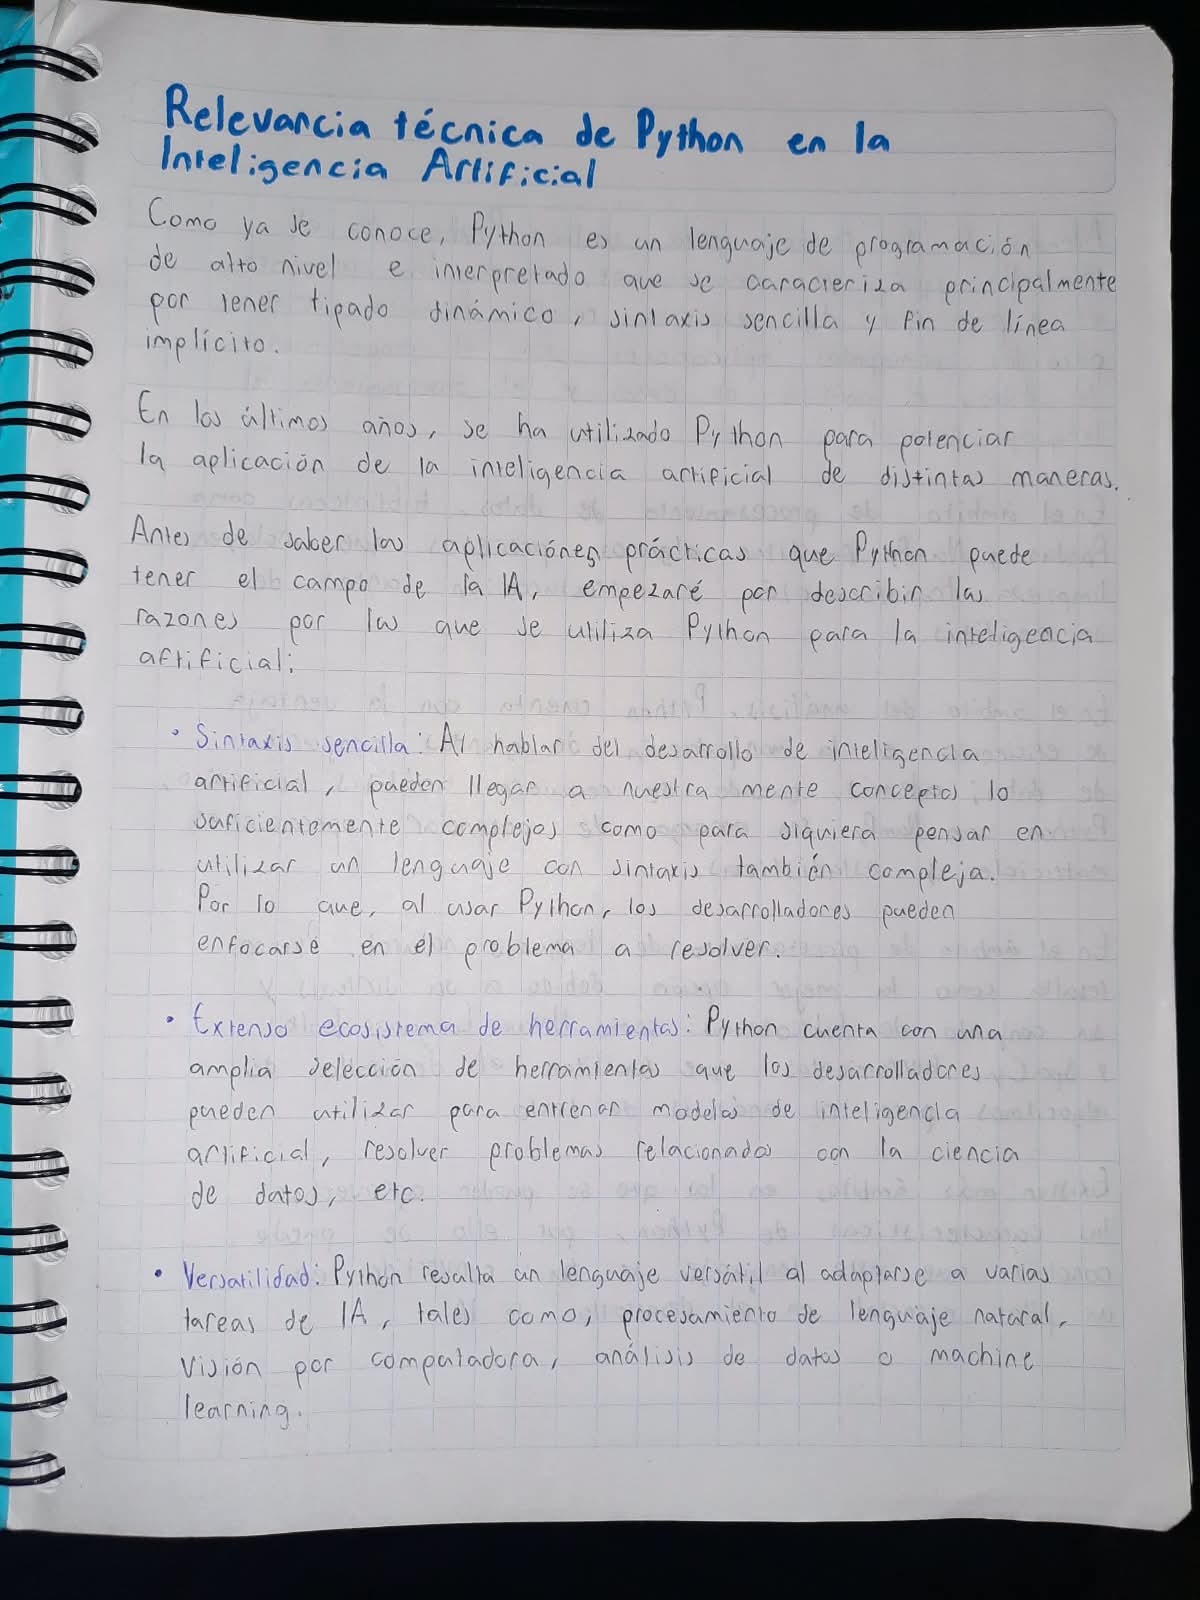
\includegraphics[width=\textwidth]{img/texto_1.jpeg}
    \caption{Primer parte del texto}
    \label{fig:texto_1}
\end{figure}

\begin{figure}[h]
    \centering
    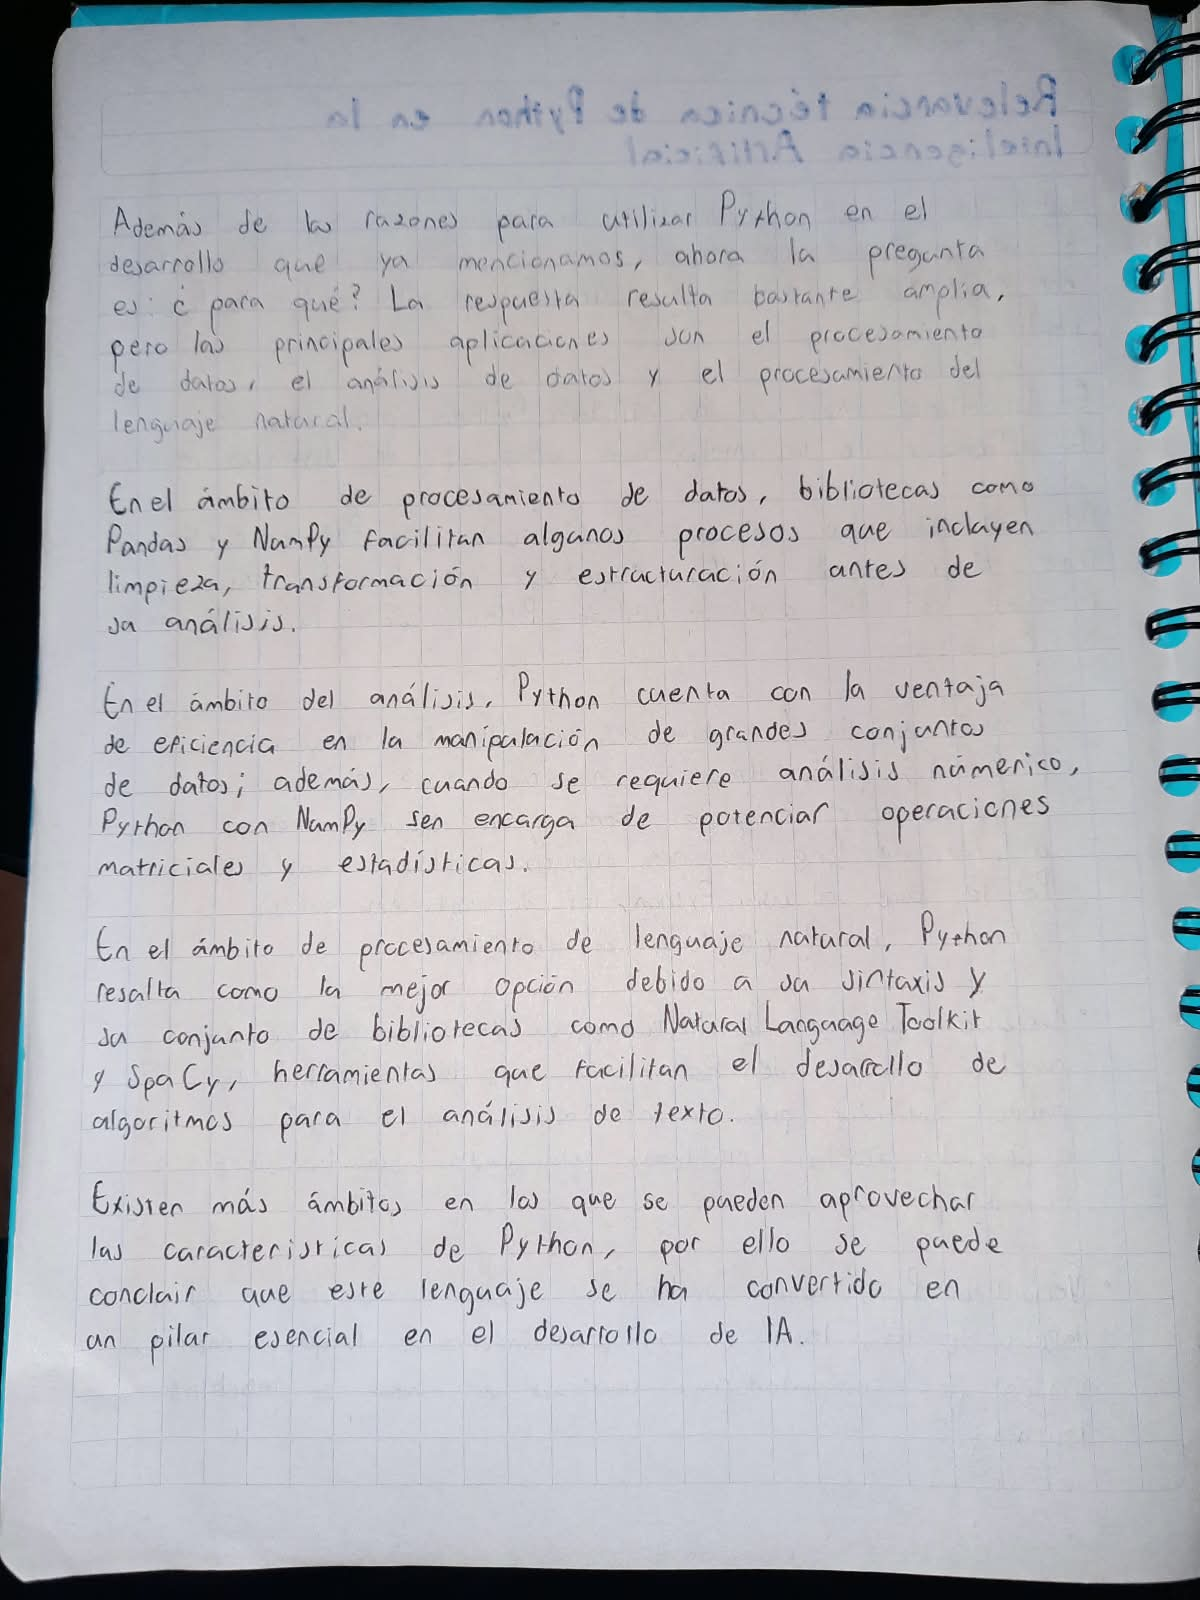
\includegraphics[width=\textwidth]{img/texto_2.jpeg}
    \caption{Segunda parte del texto}
    \label{fig:texto_2}
\end{figure}

\end{document}
